%%%%%%%%%%%%%%%%%%%%%%%%%
%%  Capítulo 3: Modelado y simulacion de metamateriales  %%
%%%%%%%%%%%%%%%%%%%%%%%%%

%%%%
\section{Análisis de estructuras periódicas}
\label{sec_estructuras_periodicas}
%%%%
\lipsum
% Libro de rahmat. Pagina 59.
%%%%
\section{Análisis de estructuras planares propuestas}
\label{sec_estructuras_propuestas}
%%%%
\lipsum
\lipsum
% Comentar cómo se logró periodicidad, vinculando las fases.
%%%%
\section{Estudio de estructuras mediante TLM}
\label{sec_estudio_tlm}
%%%%
\lipsum
%Pasos: Barchloui: Simulation of FSS surfaces using 3d TLM, 2003. Primer paper de un librito. Buena explciaci{on.}
% Paper importante: Hoefer 1985. Johns, 1971.
% Leer Janyani, Paul, TLM modelling of nonlinear optical effects in fibre bragg gratings, 2004.
% Kim Kim Kang, Yook: Modeling and analysis of ebg in power distribution networks.
% sadiku

%%%%
\subsection{Algoritmo utilizando programación orientada a objetos}
\label{subsec_estudio_tlm}
%%%%
La simulación se corre a través de un \textit{script} de Python, donde se establecen las condiciones de la simulación en forma manual, editando el archivo \textsc{tlm.py}, para comenzar una simulación, guardarla en un archivo, o leer una previa desde el disco rígido. Además, se permite determinar si se utilizarán las capacidades de acople entre elementos, la cantidad de tiempos a simular y las frecuencias superior e inferior de análisis. La frecuencia superior de análisis se debe seleccionar con cuidado, dado que como la discretización espacial y temporal de TLM están vinculadas por la velocidad de propagación de una onda electromagnética en el medio, la primera deberá asegurar que la segunda permita asegurar las condiciones del teorema de Nyquist.

La entrada de datos se realiza a través de un archivo con formato \textsc{.PGM}, que establece una matriz de pixeles, cada uno con un valor, entre 1 y 255, donde 1 representa el negro, 255 el blanco, y los valores intermedios corresponden a una escala de grises. El archivo se puede generar a partir de un programa de edición de imágenes, lo que facilita la creación de estructuras a simular, ya que la misma sólo debe ser dibujada. Si la imagen creada ocupa una mayor cantidad de pixeles, la granularidad espacial utilizada en la simulación será mayor, dado que existe una relación 1 a 1 entre los pixeles gráficos y la discretización utilizada. El análisis se realiza pixel a pixel, donde cada tiene un comportamiento en función de su tipo (indicado por el color que posee) y su posición respecto de los demás.

\begin{figure}[h]
	\centering
	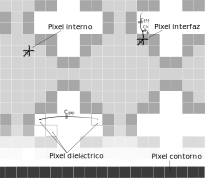
\includegraphics[width=\textwidth]{Modelado/TiposDePixel.pdf}
	\caption{Circuitos equivalentes propuestos para cada tipo de pixel.}
	\label{fig:tiposdepixeles}
\end{figure}

Existen 4 tipos de pixeles, mostrados en la figura \ref{fig:tiposdepixeles}:
\begin{enumerate}
	\item \textit{Interno}. Estos pixeles representan superficies metálicas que se encuentran en el interior de un plano conductor.
	\item \textit{Interfaz}. Estos pixeles representan superficies metálicas que se encuentran en los bordes de una estructura metálica, lo que significa que tienen vecinos que son otros pixeles de tipo metálico (de interfaz o internos) y vecinos dieléctricos. Son los pixeles que poseen la propiedad de capacidad de \textit{fringe}.
	\item \textit{Dieléctricos}. Son pixeles que representan las zonas donde no hay cobre, sino simplemente dieléctrico desnudo (en particular, FR4). Estos pixeles no participan del intercambio de energía, excepto aquellos que son vecinos de pixeles de interfaz. Cuando existe un pixel vecino interfaz, el pixel dieléctrico guarda la información de la tensión que recibe del mismo, y envía la información al pixel dieléctrico que se encuenta inmediatamente en frente, con el que se encuenta vinculado capacitivamente.
	\item \textit{Contorno}. Los pixeles contorno tienen un comportamiento especial. Pueden intentar simular una superficie perfectamente adaptada, o una superficie metálica, en función de las necesidades de la simulación. Se ubican en el borde de la imagen \textit{.pgm} creada, para que actúen como el borde del espacio de simulación.
\end{enumerate}

Los pixeles están ordenados en una superficie, creada al momento de leer la imagen \textsc{.pgm} del disco. En función de los colores, se crean, para cada pixel gráfico y en base a su color, objetos de clase "Pixel" de alguno de los tipos previamente nombrados, y se ubican en una matriz que se carga en memoria, y que tiene comportamientos diferentes según el tipo de pixel representado.

Capa pixel tiene una capacidad y varias inductancias asociadas (una para cada dirección), descriptas en base a las ecuaciones \ref{eq:Cp_Lp}, a partir de las cuales se puede obtener una impedancia:


\begin{align}
L_{inn} &= \mu_0 h /2 \\
C_{inn} &= \frac{\epsilon_r \epsilon_0 l^2}{h} \\
Z_{inn} &= \sqrt{L_{inn} / C_{inn}}
\end{align}

Los pixeles interfaz poseen, además, una capacidad de \textit{fringe}, que se relaciona al comportamiento no-TEM de las líneas de campo cerca de los bordes de las estructuras \textit{microstrip}, mostrado en la figura \ref{fig:microstrip-campos}. Esta capacidad de \textit{fringe} se suma a la capacidad de placas planas paralelas propia del pixel en la dirección correspondiente (la dirección cuyo vecino es una pixel de tipo dieléctrico). La expresión de la capacidad de \textit{fringe} para cada celda es la siguiente \cite{ThummWiesbeck:CharacteristicImpedance}:

\begin{equation}
	C_{fr} = \frac{\epsilon_0 \epsilon_r} {\pi} \ln (2 \pi e^{\frac{prof}{2 h} + 0.92})
\end{equation}

Para el análisis de transferencia entre un punto y otro de la estructura, se debe fijar una posición de entrada y una posición de salida, cuya tensión, para cada tiempo, deberá ser almacenada.

Una vez creada la matriz a partir de la información obtenida de la imagen, se debe establecer una tensión inicial en el nodo de entrada. Se puede establecer un $\delta(t)$ de tensión, de manera que se fija el valor de tensión inicial y luego se lo deja libre para todos los tiempos posteriores. También puede establecerse un seno y un pulso Gaussiano, que permite una excitación limitada en frecuencia \cite{Barthia:Handbook}. En todos los casos, la tensión impuesta puede sumarse a la tensión que obtiene naturalmente el nodo en los tiempos posteriores al tiempo inicial, o puede fijarse arbitrariamente para todos los tiempos, en función de las necesidades. 

Al momento de crear la superficie, además, se realizan dos acciones previas a la simulación:
\begin{figure}[h]
	\centering
	\includegraphics[width=0.9\textwidth]{Modelado/ProcesoProfundidad.pdf}
	\caption{Cálculo de las distintas capacidades de acople para los pixeles que participan del cálculo numérico. Para un caso particular se muestran las capacidades de acople asociadas a los pixeles enfrentados por un \textit{gap}.}
	\label{fig:calculoCapacidadTLM}
\end{figure}

\begin{enumerate}
	\item \textbf{Vincular capacitivamente los bordes de las estructuras metálicas}, como se indica en la figura \ref{fig:calculoCapacidadTLM}. Para esto se toman todos los bordes de las estructuras metálicas (los pixeles de tipo Interfaz), y se recorre horizontal y verticalmente la matriz, una vez por dirección, vinculando los bordes interfaz de a pares, teniendo en cuenta que aquellos pixeles de interfaz que corresponden a la misma estructura o a la misma celda unitaria (a la misma isla metálica) no deben ser vinculados. Por cada par encontrado, se obtiene la capacidad de acople, $C_{gt}$, utilizando la expresión \ref{eq:cgap-y-lgap}. En esta expresión, $a$ es el tamaño de las islas metálicas y $g$ representa la distancia entre las islas conductoras. El valor de $s$, en tanto, representa la longitud del $gap$, que se obtiene calculando la cantidad de pixeles enfrentado a distancia constante que existen (paso 1 en la figura). Hecho esto, considerando todos los pixeles a uno y otro lado del \textit{gap}, se busca la "profundidad" de la celda, $u$, que no es más que la cantidad de pixeles metálicos detrás de los pixeles frontera que pueden hallarse simultáneamente a ambos lados del \textit{gap}, manteniendo al cantidad longitudinal de pixeles metálicos del borde (paso 2 en la figura). Así, el valor de $a$ queda representado por, aproximadamente, $2*u+g$, con $u$ en unidades de metro. El valor de la capacidad total de acople se divide entre la cantidad de pixeles que participan del cálculo, de manera que a cada uno se le asigna una capacidad $C_g$, como se indica en la figura para los pixeles de color rojo. La vinculación se realiza entre pixeles dieléctricos adyacentes a los pixeles frontera en cuestión, de forma que los pixeles frontera no participen del intercambio de información con otros pixeles.
	
	\item \textbf{Calcular las matrices S de cada pixel.} Las matrices S son las matrices que, multiplicadas por un vector de tensiones incidentes, $V_i$, devuelven un vector de igual dimensión de tensiones reflejadas, $V_r$. Cada uno de los elementos de estos vectores representan una dirección (arriba, abajo, derecha, izquierda) de la celda unitaria. Las expresiones de la matriz S son las mostradas en la ecuación \ref{eq:matriz-s-expresiones}:
	\begin{subequations}
		\label{eq:matriz-s-expresiones}
		\begin{align}
			S_{i,i} = \frac{Z_{j}||Z_{k}||Z_{l} -Z_{i}}{Z_{j}||Z_{k}||Z_{l} +Z_{i}} \\
			S_{j,i} = \frac{2 Z_{j}||Z_{k}||Z_{l}}{Z_{j}||Z_{k}||Z_{l} +Z_{i}}
		\end{align}
	\end{subequations}
	Además, se pueden establecer pérdidas para el transporte de tensión de un pixel a otro, de manera que se puedan simular, de forma simplificada, las pérdidas por conductividad.
	
	Los pixeles de tipo dieléctrico no poseen matriz S, debido a que en su mayoría no tendrán información de tensión incidente.
\end{enumerate}
	
La simulación es de tipo TLM, donde existe una tensión inicial impuesta como condición inicial, y elegida previamente al cálculo. A partir de la tensión ubicada en uno de los nodos, se calcula, en cada tiempo discreto, el valor de las tensiones incidentes a cada nodo, y a partir de las mismas, se calculan las tensiones reflejadas en todas las direcciones (\textit{scattering}), sumándose los efectos en todas ellas.

\begin{figure}[h]
	\centering
	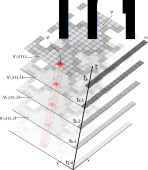
\includegraphics[width=0.9\textwidth]{Modelado/ConceptoMatrizProgresoTiempo.pdf}
	\caption{Estructura de la matriz que se guarda y se lee del disco rígido. La estructura posee todas las tensiones calculadas para cada tiempo y para cada pixel en particular.}
	\label{fig:EstructuraTiemposMatrizNumpy}
\end{figure}

El resultado arrojado por la simulación será un archivo, de formato .npy, que es una matriz tridimensional, que puede ser considerada como un apilamiento, de tamaño igual a la cantidad de tiempos simulados, de matrices bidimensionales con tamaño igual al de la estructura, como se muestra en la figura \ref{fig:EstructuraTiemposMatrizNumpy}. En cada una de estas últimas matrices bidimensionales, cada elemento posee un valor, que no es más que la tensión vista en ese nodo en el tiempo al que la matriz bidimensional corresponde. De ser necesario, se pueden establecer los parámetros de una ventana de Hanning para disminuir el comportamiento espúreo de alta frecuencia debido a la limitación en tiempo de la señal de salida.